\documentclass{standalone}
\usepackage{tikz}
\usetikzlibrary{patterns, positioning}
\usepackage[sfdefault]{ClearSans} %% option 'sfdefault' activates Clear Sans as the default text font
\usepackage[T1]{fontenc}

\begin{document}
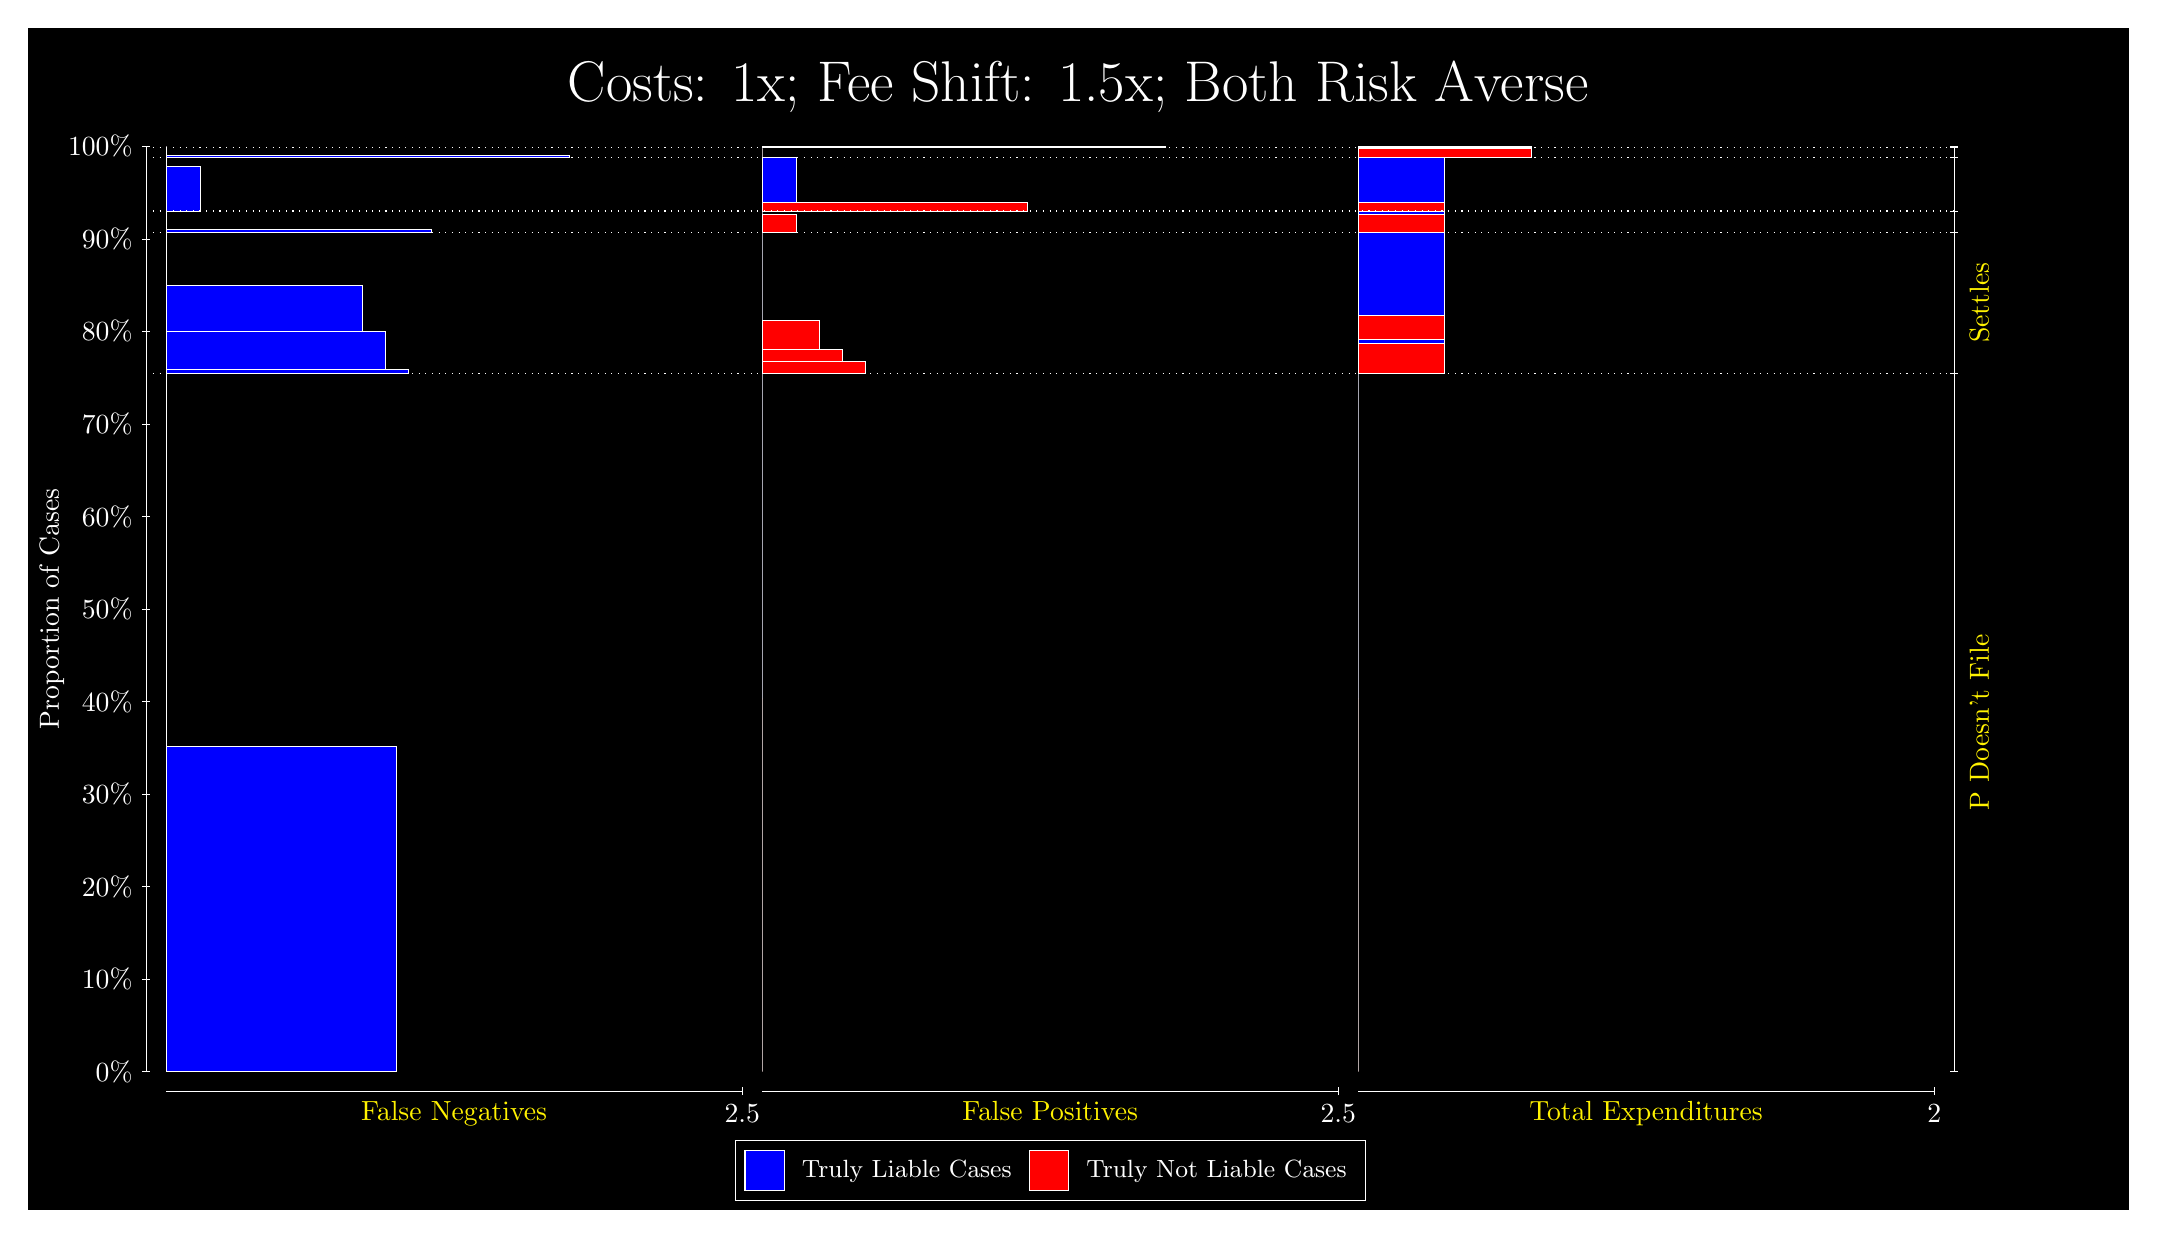
\begin{tikzpicture}
\draw[fill=black] (0,0) rectangle (26.667,15);
\draw[text=white] (0,13.5) rectangle (26.667,15) node[midway] {\huge Costs: 1x; Fee Shift: 1.5x; Both Risk Averse};
\draw[white, very thin] (1.5,1.75) -- (1.5,13.5);
\node[rotate=90, text=white, anchor=center] at (0.3, 7.625) {Proportion of Cases};
\draw[white, very thin] (1.45,1.75) -- (1.55,1.75);
\node[text=white, anchor=east] at (1.45, 1.75) {0\%};
\draw[white, very thin] (1.45,2.925) -- (1.55,2.925);
\node[text=white, anchor=east] at (1.45, 2.925) {10\%};
\draw[white, very thin] (1.45,4.1) -- (1.55,4.1);
\node[text=white, anchor=east] at (1.45, 4.1) {20\%};
\draw[white, very thin] (1.45,5.275) -- (1.55,5.275);
\node[text=white, anchor=east] at (1.45, 5.275) {30\%};
\draw[white, very thin] (1.45,6.45) -- (1.55,6.45);
\node[text=white, anchor=east] at (1.45, 6.45) {40\%};
\draw[white, very thin] (1.45,7.625) -- (1.55,7.625);
\node[text=white, anchor=east] at (1.45, 7.625) {50\%};
\draw[white, very thin] (1.45,8.8) -- (1.55,8.8);
\node[text=white, anchor=east] at (1.45, 8.8) {60\%};
\draw[white, very thin] (1.45,9.975) -- (1.55,9.975);
\node[text=white, anchor=east] at (1.45, 9.975) {70\%};
\draw[white, very thin] (1.45,11.15) -- (1.55,11.15);
\node[text=white, anchor=east] at (1.45, 11.15) {80\%};
\draw[white, very thin] (1.45,12.325) -- (1.55,12.325);
\node[text=white, anchor=east] at (1.45, 12.325) {90\%};
\draw[white, very thin] (1.45,13.5) -- (1.55,13.5);
\node[text=white, anchor=east] at (1.45, 13.5) {100\%};

\draw[white, very thin] (24.457,1.75) -- (24.457,13.5);
\draw[white, very thin] (24.407,1.75) -- (24.507,1.75);
\node[anchor=west] at (24.407, 1.75) {};
\draw[white, very thin] (24.407,10.619) -- (24.507,10.619);
\node[anchor=west] at (24.407, 10.619) {};
\draw[white, very thin] (24.407,12.408) -- (24.507,12.408);
\node[anchor=west] at (24.407, 12.408) {};
\draw[white, very thin] (24.407,12.678) -- (24.507,12.678);
\node[anchor=west] at (24.407, 12.678) {};
\draw[white, very thin] (24.407,13.363) -- (24.507,13.363);
\node[anchor=west] at (24.407, 13.363) {};
\draw[white, very thin] (24.407,13.489) -- (24.507,13.489);
\node[anchor=west] at (24.407, 13.489) {};
\draw[white, very thin] (24.407,13.5) -- (24.507,13.5);
\node[anchor=west] at (24.407, 13.5) {};

\draw[white, very thin, fill=blue] (1.75,1.75) rectangle (4.6775,5.8777);
\draw[white, very thin, fill=red] (1.75,5.8777) rectangle (1.75,10.619);
\draw[white, very thin, fill=blue] (1.75,10.619) rectangle (4.8239,10.674);
\draw[white, very thin, fill=blue] (1.75,10.674) rectangle (4.5312,11.15);
\draw[white, very thin, fill=blue] (1.75,11.15) rectangle (4.2384,11.731);
\draw[white, very thin, fill=red] (1.75,11.731) rectangle (1.75,12.408);
\draw[white, very thin, fill=blue] (1.75,12.408) rectangle (5.1167,12.447);
\draw[white, very thin, fill=red] (1.75,12.447) rectangle (1.75,12.678);
\draw[white, very thin, fill=blue] (1.75,12.678) rectangle (2.1891,13.251);
\draw[white, very thin, fill=red] (1.75,13.251) rectangle (1.75,13.363);
\draw[white, very thin, fill=blue] (1.75,13.363) rectangle (6.8732,13.381);
\draw[white, very thin, fill=red] (1.75,13.381) rectangle (1.75,13.489);
\draw[white, very thin, fill=red] (1.75,13.489) rectangle (1.75,13.495);
\draw[white, very thin, fill=blue] (1.75,13.495) rectangle (1.75,13.5);
\draw[white, very thin, fill=red] (9.3189,1.75) rectangle (9.3189,6.4918);
\draw[white, very thin, fill=blue] (9.3189,6.4918) rectangle (9.3189,10.619);
\draw[white, very thin, fill=red] (9.3189,10.619) rectangle (10.636,10.766);
\draw[white, very thin, fill=red] (9.3189,10.766) rectangle (10.344,10.922);
\draw[white, very thin, fill=red] (9.3189,10.922) rectangle (10.051,11.296);
\draw[white, very thin, fill=blue] (9.3189,11.296) rectangle (9.3189,12.408);
\draw[white, very thin, fill=red] (9.3189,12.408) rectangle (9.758,12.638);
\draw[white, very thin, fill=blue] (9.3189,12.638) rectangle (9.3189,12.678);
\draw[white, very thin, fill=red] (9.3189,12.678) rectangle (12.686,12.79);
\draw[white, very thin, fill=blue] (9.3189,12.79) rectangle (9.758,13.363);
\draw[white, very thin, fill=red] (9.3189,13.363) rectangle (9.3189,13.471);
\draw[white, very thin, fill=blue] (9.3189,13.471) rectangle (9.3189,13.489);
\draw[white, very thin, fill=red] (9.3189,13.489) rectangle (14.442,13.495);
\draw[white, very thin, fill=blue] (9.3189,13.495) rectangle (11.515,13.5);
\draw[white, very thin, fill=red] (16.888,1.75) rectangle (16.888,6.4918);
\draw[white, very thin, fill=blue] (16.888,6.4918) rectangle (16.888,10.619);
\draw[white, very thin, fill=red] (16.888,10.619) rectangle (17.986,10.994);
\draw[white, very thin, fill=blue] (16.888,10.994) rectangle (17.986,11.049);
\draw[white, very thin, fill=red] (16.888,11.049) rectangle (17.986,11.351);
\draw[white, very thin, fill=blue] (16.888,11.351) rectangle (17.986,12.408);
\draw[white, very thin, fill=red] (16.888,12.408) rectangle (17.986,12.638);
\draw[white, very thin, fill=blue] (16.888,12.638) rectangle (17.986,12.678);
\draw[white, very thin, fill=red] (16.888,12.678) rectangle (17.986,12.79);
\draw[white, very thin, fill=blue] (16.888,12.79) rectangle (17.986,13.363);
\draw[white, very thin, fill=red] (16.888,13.363) rectangle (19.083,13.471);
\draw[white, very thin, fill=blue] (16.888,13.471) rectangle (19.083,13.489);
\draw[white, very thin, fill=red] (16.888,13.489) rectangle (19.083,13.495);
\draw[white, very thin, fill=blue] (16.888,13.495) rectangle (19.083,13.5);
\draw[white, dotted] (1.5,10.619) -- (24.457,10.619);
\draw[white, dotted] (1.5,12.408) -- (24.457,12.408);
\draw[white, dotted] (1.5,12.678) -- (24.457,12.678);
\draw[white, dotted] (1.5,13.363) -- (24.457,13.363);
\draw[white, dotted] (1.5,13.489) -- (24.457,13.489);
\draw[white, very thin] (1.75,1.5) -- (9.0689,1.5);
\node[text=yellow, anchor=north] at (5.4094, 1.5) {False Negatives};
\draw[white, very thin] (9.0689,1.45) -- (9.0689,1.55);
\node[text=white, anchor=north] at (9.0689, 1.45) {2.5};

\draw[white, very thin] (9.3189,1.5) -- (16.638,1.5);
\node[text=yellow, anchor=north] at (12.978, 1.5) {False Positives};
\draw[white, very thin] (16.638,1.45) -- (16.638,1.55);
\node[text=white, anchor=north] at (16.638, 1.45) {2.5};

\draw[white, very thin] (16.888,1.5) -- (24.207,1.5);
\node[text=yellow, anchor=north] at (20.547, 1.5) {Total Expenditures};
\draw[white, very thin] (24.207,1.45) -- (24.207,1.55);
\node[text=white, anchor=north] at (24.207, 1.45) {2};

\node[text=yellow, centered, rotate=90] at (24.777, 6.1847) {P Doesn't File};
\node[text=yellow, centered, rotate=90] at (24.777, 11.514) {Settles};





\draw (12.978300999999998,1.5) node[draw=none] (baseCoordinate) {};
\begin{scope}[align=center]
        \matrix[scale=0.5, draw=white, below=0.5cm of baseCoordinate, nodes={draw}, column sep=0.1cm]{
            \node[rectangle, draw, minimum width=0.5cm, minimum height=0.5cm, fill=blue] {}; &
            \node[draw=none, font=\small, text=white] (B) {Truly Liable Cases}; &
            \node[rectangle, draw, minimum width=0.5cm, minimum height=0.5cm, fill=red] {}; &
            \node[draw=none, font=\small, text=white] (B) {Truly Not Liable Cases}; \\
            };
\end{scope}

\end{tikzpicture}
\end{document}